\section{Prototipo del robot}

El proyecto comenzó con el análisis de una serie de proyectos anteriores llevados a cabo en el Laboratorio de Arquitectura de Computadoras. El Hermes III, la última versión desarrollada, incorporó mejoras respecto a modelos anteriores, destacándose la inclusión del Sistema Operativo ROS para Linux y el sensor Kinect. Su principal innovación fue la implementación del algoritmo SLAM, que permite al robot mapear su entorno al mismo tiempo que localizarse en él. \cite{micolini2022hermes} Todo el sistema funciona sobre una placa $NVIDIA\ Jetson\ TK1$, que ofrece un alto rendimiento computacional pero encarece el producto.

\begin{table}[htpb]
	\begin{center}
    	\begin{tabular} {
        	| >{\centering\arraybackslash}m{2.2cm}
        	| >{\centering\arraybackslash}m{2.65cm}
        	| >{\centering\arraybackslash}m{2.65cm} |}
        	\hline \rowcolor{test_header_color}
            	Caracteristica & ESP-32 & NVIDIA Jetson TK1\\
        	\hline
            	Procesador & Xtensa LX6 & ARM Cortex A15 \\
        	\hline
            	Frecuencia CPU & 240 MHz & 2,3 GHz \\
        	\hline
            	WiFi/Bluetooth & Si & Requiere módulo externo \\
        	\hline
            	Periféricos & {Wi-Fi, Bluetooth, ADC, DAC, SPI, I2C, UART, PWM, GPIOs, SD/MMC, contador de pulsos, Timers} & {USB 3.0/2.0, HDMI, Ethernet, SATA, SD/MMC, PCIe x4, GPIOs, I2C, SPI, UART, PWM, soporte para CUDA} \\
        	\hline
            	Consumo activo & 160-250 mW & 10-12 W \\
        	\hline
            	Modo bajo consumo & Si & No \\
        	\hline
            	Sistema Operativo & FreeRTOS & ROS \\
        	\hline
            	Costo estimado (USD) & \$10 & \$150 \\
        	\hline
    	\end{tabular}
	\caption{Comparativa entre ESP32 y NVIDIA Jetson TK1}
	\label{tab:comparativa_esp32_jetson}
	\end{center}
\end{table}

Por ello determinamos necesario replantear el plan, pero manteniendo el sistema de locomoción omnidireccional, de modo que elegimos utilizar una placa de desarrollo $ESP32$ para el control principal, siendo esta mucho más accesible que la $NVIDIA\ Jetson\ TK1$.\cite{kolban2017kolban} Sobre ella montamos un Sistema Operativo de tiempo real FreeRTOS y donde implementamos las tareas y mecanismos de control. \cite{barry2016mastering} En comparación con el modelo anterior del robot, destacamos el bajo precio que conlleva la implementación, ya que los componentes son de fácil acceso, lo que además posibilita la creación de una flota de los mismos. En la Tabla \ref{tab:comparativa_esp32_jetson} se muestra la comparativa entre el microcontrolador $ESP32$ y la placa $Jetson$ utilizada en el Hermes III donde observamos una reducción del coste en un $93\%$.

Dada la necesidad de controlar la velocidad de los motores, es necesario medir esta velocidad. Para solventar ese problema desarrollamos un medidor de RPM utilizando un opto-acoplador de ranura y los módulos contadores de pulso de la ESP32. Por limitaciones del diseño del medidor de RPM, el error es considerable al medir bajas RPM ($<60[RPM]$), por lo que iteramos sobre diversas técnicas para la medición de RPM hasta converger a la actual. La misma consiste en acumular cuentas hasta que se tiene un valor suficiente para permitir el cálculo de RPM en las últimas N mediciones. Para esto se tiene una ventana deslizante que toma más o menos muestras acumuladas dependiendo del valor de cuentas en el último $\Delta T$.

Además, integramos una comunicación bidireccional inalámbrica, aprovechando el módulo WiFi de la placa y usando el protocolo MQTT para el envío y recepción de información y comandos.

\subsection{Sistema de control}

Desarrollamos un sistema de control utilizando un controlador PID aditivo como el descrito en la Figura \ref{fig:pidaditivo}. \cite{ogatacontrol}

\begin{figure}[htpb]
	\hspace{-1cm}
	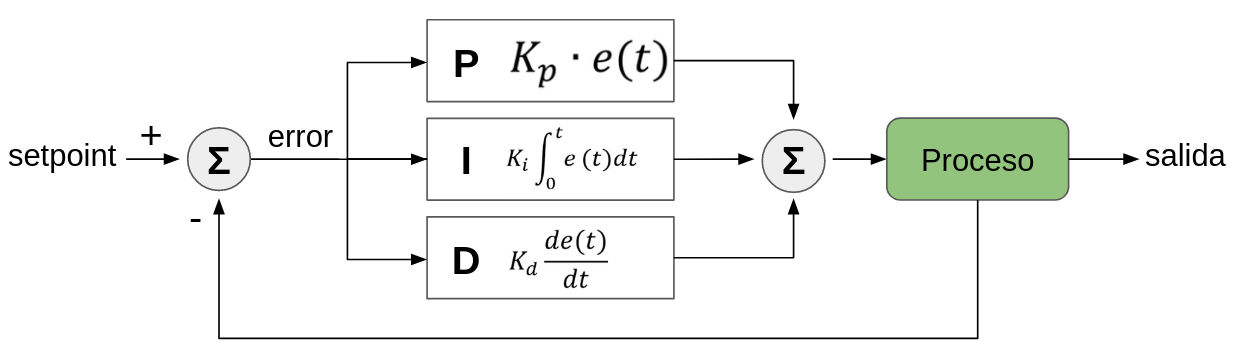
\includegraphics[width=1.1\linewidth]{images/pid_aditivo}
	\caption{PID aditivo}
	\label{fig:pidaditivo}
\end{figure}

Obtuvimos los coeficientes del controlador PID con distintas iteraciones empíricas, los resultados se expresan en la Tabla \ref{coeficientes_pid}:

\begin{table}[htpb]
	\begin{center}
    	\begin{testtableformat}
        	\hline \rowcolor{test_header_color}
            	Coeficiente	& Valor \\
        	\hline
            	Proporcional   & 16 \\
        	\hline
            	Integral   	& 7.3 \\
        	\hline
            	Derivativo 	& 0.23 \\
        	\hline
    	\end{testtableformat}
    	\caption{Coeficientes obtenidos del controlador PID}
    	\label{coeficientes_pid}
	\end{center}
\end{table}

%%%%%%%%%%%%%%%%%%%%%%%%%%%%%%%%%%%%%%%%%%%%%%%%%%%%%%%%%%%%%%%%%%%%%%%%%%%%%%%%%%%%%%%%%%
%%%%%%%%%%%%%%%%%%%%%%%%%%%%%%%%%%%%%%%%%%%%%%%%%%%%%%%%%%%%%%%%%%%%%%%%%%%%%%%%%%%%%%%%%%

\subsection{Modelo Cinemático}
Un modelo cinemático aplicado a nuestro robot omnidireccional permite producir movimientos rectos y curvos sobre el plano. \cite{rijalusalamkinematics}
Se utilizan ecuaciones cinemáticas directas e inversas para relacionar las velocidades de las ruedas con el movimiento global del robot. La cinemática directa permite calcular las velocidades necesarias en cada rueda para lograr un movimiento deseado, mientras que la inversa, a partir de las velocidades angulares medidas, permite deducir el vector de movimiento real del robot, lo cual es esencial para el control y navegación. \cite{tzafestas2013introduction} \cite{islassistcontrolomni}
Estas ecuaciones consideran la disposición geométrica y orientación fija de las ruedas, que en este caso son de tipo Omni-wheel todas de radio $r_i = 5,08 cm\ (2'')$, mientras que el radio del cuerpo del robot es de $L = 14cm\ (5,51'')$. Lo anterior está representado en la Figura \ref{fig:vectoresrobotmodelocinem}.

\begin{figure}[htpb]
	\centering
	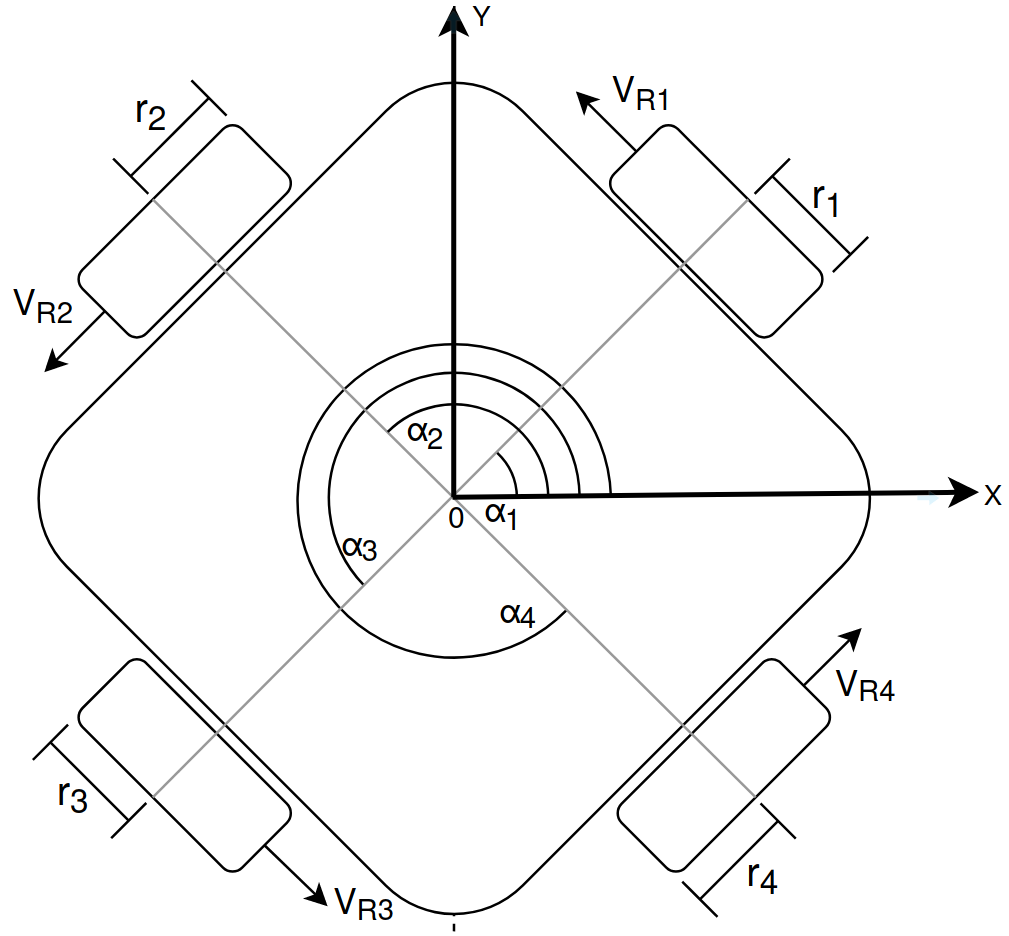
\includegraphics[width=0.95\linewidth]{images/modelo_cinematico_robot_ruedas.png}
	\caption{Descomposición de vectores del robot y orientación de las ruedas}
	\label{fig:vectoresrobotmodelocinem}
\end{figure}

La matriz cinemática inversa (IK) toma como entrada $V_x, V_y$ expresadas en $[m/seg]$ y $V_\theta$ expresada en $[RPM]$. Por otra parte, la salida $\omega_n$ se determina en $[rad/seg]$:

\begin{equation}
	\begin{bmatrix} w_1 \\ w_2 \\ w_3 \\ w_4 \\ \end{bmatrix} = IK \cdot \begin{bmatrix} V_x \\ V_y \\ V_\theta \\ \end{bmatrix}
\end{equation}

Al desarrollar para nuestro caso, obtenemos que la matriz cinemática inversa puede expresarse como:

\begin{equation}
	IK =
	\frac{1}{r}
	\cdot
	\begin{bmatrix}
    	{-sen(\alpha_1)} & {cos(\alpha_1)} & L \\
    	{-sen(\alpha_2)} & {cos(\alpha_2)} & L \\
    	{-sen(\alpha_3)} & {cos(\alpha_3)} & L \\
    	{-sen(\alpha_4)} & {cos(\alpha_4)} & L \\
	\end{bmatrix}
	\label{ec:matriz_cinematica}
\end{equation}

Reemplazando en la ecuación \ref{ec:matriz_cinematica}, obtenemos:
\begin{equation}
	\begin{bmatrix}
    	w_1 \\ w_2 \\ w_3 \\ w_4 \\
	\end{bmatrix} = \frac{1}{r} \cdot
	\begin{bmatrix}
    	{-sen(\frac{\pi}{4})} & {cos( \frac{\pi}{4})} & L \\
    	{-sen(\frac{3\pi}{4})} & {cos(\frac{3\pi}{4})} & L \\
    	{-sen(\frac{5\pi}{4})} & {cos(\frac{5\pi}{4})} & L \\
    	{-sen(\frac{7\pi}{4})} & {cos(\frac{7\pi}{4})} & L \\
	\end{bmatrix} \cdot
	\begin{bmatrix} V_x \\ V_y \\ V_\theta \\
	\end{bmatrix}
\end{equation}

Dado que en ciertos casos es preferible utilizar setpoints de velocidad para las ruedas expresados en $[RPM]$, debemos hacer una conversión a esa unidad. Por lo que planteamos una matriz que convierta los valores de las dos primeras columnas de la matriz cinemática, que son los coeficientes que nos interesa convertir a $[RPM]$, dado que los de la última columna ya están expresados en esa unidad.

\begin{equation}
	\begin{bmatrix} w_1 \\ w_2 \\ w_3 \\ w_4 \\
	\end{bmatrix} = IK \cdot
	\begin{bmatrix}
    	{\frac{60}{2 \pi}} & {0} & {0} \\
    	{0} & {\frac{60}{2 \pi}} & {0} \\
    	{0} & {0} & {1}            	\\
	\end{bmatrix} \cdot
	\begin{bmatrix} V_x \\ V_y \\ V_\theta \\
	\end{bmatrix}
\end{equation}

\subsection{Compensación del Modelo Cinemático}
Para obtener el vector de velocidad lineal real que efectivamente realiza el robot y poder aplicar correcciones sobre la misma, hacemos uso de las mediciones de velocidad angular en cada rueda, que se ingresan a la ecuación cinemática directa \ref{ec:matriz_cinematica_directa}. Esta matriz se obtiene a partir de la pseudoinversa de la matriz cinemática inversa. \cite{islassistcontrolomni}

Expresamos la conversión para obtener el vector lineal en base a las velocidades de las ruedas expresadas en $[rad/seg]$:

\begin{equation}
	\begin{bmatrix}
    	V_x \\ V_y \\ V_\theta \\
	\end{bmatrix} = DK \cdot
	\begin{bmatrix}
    	w_1 \\ w_2 \\ w_3 \\ w_4 \\
	\end{bmatrix}
	\label{ec:matriz_cinematica_directa}
\end{equation}

Luego, al realizar la pseudoinversa de la matriz $IK$ obtenemos $DK$:

\begin{equation}
	DK = r \cdot
	\begin{bmatrix}
    	{\frac{-sen(\alpha_1)}{2}} & {\frac{-sen(\alpha_2)}{2}} & {\frac{-sen(\alpha_3)}{2}} & {\frac{-sen(\alpha_4)}{2}} \\
    	{\frac{cos(\alpha_1)}{2}}  & {\frac{cos(\alpha_2)}{2}}  & {\frac{cos(\alpha_3)}{2}}  & {\frac{cos(\alpha_4)}{2}}  \\
    	{\frac{1}{4L}}  & {\frac{1}{4L}}  & {\frac{1}{4L}}  & {\frac{1}{4L}}  \\
	\end{bmatrix}
	\label{ec:dk}
\end{equation}

Al reemplazar en la ecuación \ref{ec:dk} tenemos:

\small{
\begin{equation}
	\hspace{-1.1cm}
	\begin{bmatrix}
    	V_x \\ V_y \\ V_\theta \\
	\end{bmatrix} = r \cdot
	\begin{bmatrix}
    	{\frac{-sen(\alpha_1)}{2}} & {\frac{-sen(\alpha_2)}{2}} & {\frac{-sen(\alpha_3)}{2}} & {\frac{-sen(\alpha_4)}{2}} \\
    	{\frac{cos(\alpha_1)}{2}}  & {\frac{cos(\alpha_2)}{2}}  & {\frac{cos(\alpha_3)}{2}}  & {\frac{cos(\alpha_4)}{2}}  \\
    	{\frac{1}{4L}}  & {\frac{1}{4L}}  & {\frac{1}{4L}}  & {\frac{1}{4L}}  \\
	\end{bmatrix} \cdot
	\begin{bmatrix}
    	w_1 \\ w_2 \\ w_3 \\ w_4 \\
	\end{bmatrix}
	\label{ec:velocidades_lineales}
\end{equation}
} \normalsize

La expresión \ref{ec:velocidades_lineales} toma las velocidades angulares de las ruedas en $[rad/seg]$, por lo que convertimos la entrada para que pueda ser $[RPM]$. Planteamos una matriz que solo convierta los valores de las dos primeras filas, que son los coeficientes que nos interesa convertir a $[RPM]$, dado que los de la última fila ya están expresados en esa unidad.

\begin{equation}
	\begin{bmatrix}
    	V_x \\ V_y \\ V_\theta \\
	\end{bmatrix} =
	\begin{bmatrix}
    	{\frac{2\pi}{60}} & {0} & {0}  \\
    	{0} & {\frac{2\pi}{60}} & {0} \\
    	{0} & {0} & {1} \\
	\end{bmatrix}
	\cdot
	DK
	\cdot
	\begin{bmatrix}
    	w_1 \\ w_2 \\ w_3 \\ w_4 \\
	\end{bmatrix}
\end{equation}

El desarrollo de la cinemática inversa permitió la implementación de un mecanismo para realizar la odometría del robot, es decir, medir su desplazamiento en el espacio.

Para corregir el vector de movimiento del robot planteamos una compensación mostrada en la Figura \ref{fig:diagramamodelocinemcompensado}. En primer lugar introducimos el vector deseado $(V_x[m/s], V_y[m/s], V_\theta[RPM])$ en la matriz $IK$ para obtener las velocidades de cada una de las ruedas. Luego, las mediciones de RPM de cada una de ellas ingresan en la matriz $DK$ para obtener el vector de movimiento real $(V_x'[m/s], V_y'[m/s], V_\theta'[RPM])$, que se compara con el vector deseado. El error entre ellos es inyectado en la matriz $IK$ para obtener el valor de compensación de RPM para cada rueda. Es decir, calculamos el error detectado entre el vector de movimiento deseado y el medido por la cinemática directa, de modo que determinamos las correcciones necesarias para las velocidades de las ruedas y enviamos estos valores a los actuadores de las ruedas. \cite{rijalusalamkinematics}

\begin{figure}[htpb]
	\centering
   % \hspace{-1cm}
	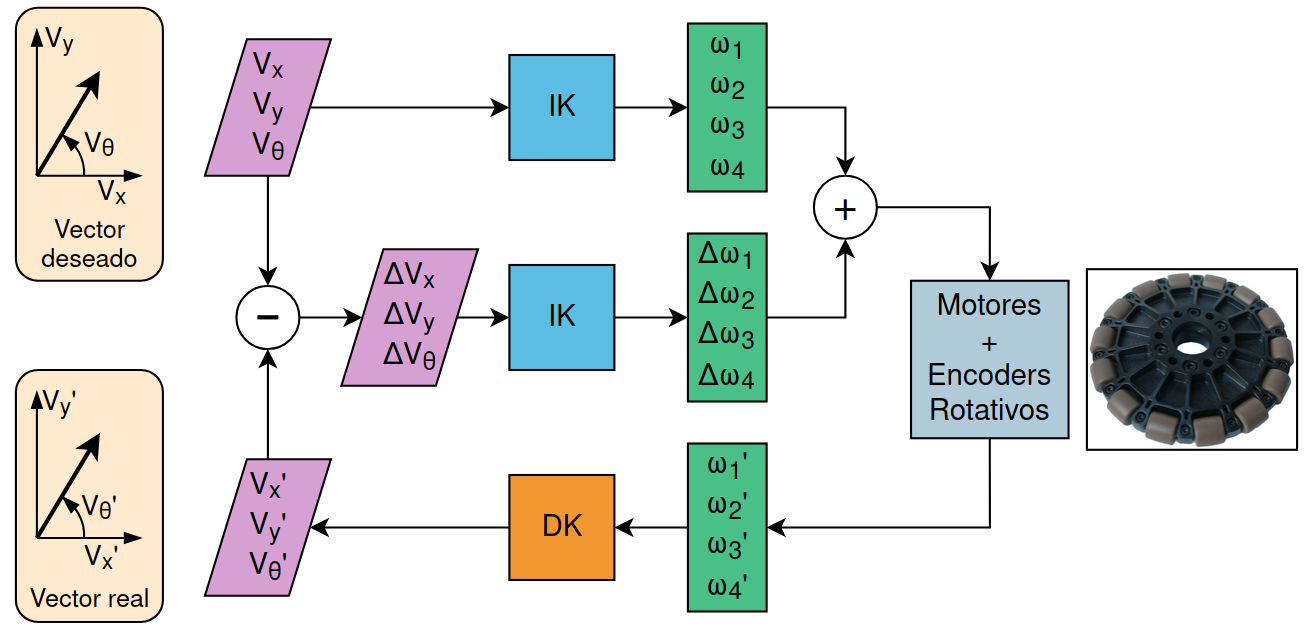
\includegraphics[width=1.0\linewidth]{images/diag_compensacion_modelo_cinem.png}
	\caption{Diagrama del Modelo Cinemático compensado}
	\label{fig:diagramamodelocinemcompensado}
\end{figure}

\subsubsection{Seguidor de línea magnético} \mbox{} \vspace{6pt}

Aunque la odometría es esencial para estimar la posición y orientación del robot, es propensa a errores acumulativos, por lo que se propone complementar su uso con un seguidor de línea. Este sistema, basado en sensores que detectan marcas en el entorno, permite al robot corregir su trayectoria al identificar desviaciones respecto a una línea de referencia. Analizamos diversas alternativas para realizar esto y optamos por un seguidor de línea magnético por su resistencia a las condiciones del entorno, bajo costo, durabilidad y bajo mantenimiento. De este modo, implementamos un mecanismo de control para llevar el desplazamiento rotacional del robot a cero, por lo que al detectar un imán se puede entender como un desplazamiento positivo o negativo sobre el mismo eje del robot, lo que significa que se alteró su orientación. Un ejemplo de esta situación se detalla en la Figura \ref{fig:deteccionimanrobot}.

\begin{figure}[htpb]
	\centering
	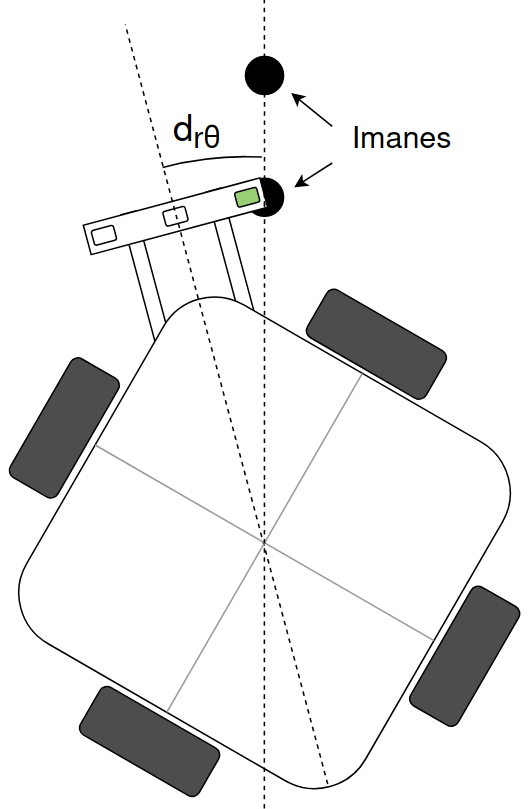
\includegraphics[width=0.55\linewidth]{images/robot_desplazamiento_angular_toca_iman.png}
	\caption{Escenario de detección de un imán}
	\label{fig:deteccionimanrobot}
\end{figure}